%!TEX root = ../../main.tex
\subsection{Intrusion Detection}
\label{sec:intrusion_detection}

Intrusion detection  system (IDS) refers to identifying malicious activity in a computer related system~\cite{phoha2002internet}. IDS may be deployed at single computers known as Host Intrusion Detection (HIDS) to large networks Network Intrusion Detection (NIDS). The classification of deep anomaly detection techniques for intrusion detection is in Figure ~\ref{sec:intrusionDetect}. IDS depending on detection method are classified into signature based or anomaly based. Using signature based IDS is not efficient to detect new attacks, for which no specific signature pattern is available, hence anomaly based detection methods are more popular. In this survey we focus on deep anomaly detection (DAD) methods and architectures eemployed in intrusion detection.

\subsubsection{Host-Based Intrusion Detection Systems (HIDS):}
 Such systems are installed software programs which monitors a single host or computer for malicious  activity or policy violations by listening to system calls or events occurring within that host ~\cite{vigna2005host}. The system call logs could be generated by programs or by user interaction resulting in logs as shown in Figure~\ref{fig:deeplogContextual}. Malicious interactions lead to execution of these system calls in different sequences. HIDS may also monitor the state of a system, its stored information, whether in Random Access Memory (RAM), in the file system, log files or elsewhere for a valid sequence, hence the length of the sequence for each program may be different.
 Deep anomaly detection (DAD) techniques applied for HIDS are required to handle the sequential nature of data. The DAD techniques have to either model the sequence data or compute similarity between sequences. Some of the successfull DAD techniques for HIDS is illustrated in Table~\ref{tab:HIDS}.

\subsubsection{Network Intrusion Detection Systems (NIDS):} NIDS systems deal with monitoring the entire network for suspicious traffic by examining each and every network packet. Owing to real-time streaming behaviour, the nature of data is synomynous to big data with high volume, velocity, variety. The network data also has a temporal aspect associated with it. Some of the successfull DAD techniques for NIDS is illustrated in Table~\ref{tab:NIDS}. This survey also lists the datasets used for evaluating the DAD intrusion detection methods proposed in Table~\ref{tab:IDSDataset}. A challenge faced by deep anomaly detection techniques in intrusion detection is that the nature of anomalies keeps changing over time as the intruders adapt their network attacks to evade the existing intrusion detection solutions.

% Begin Figure
\begin{figure*}
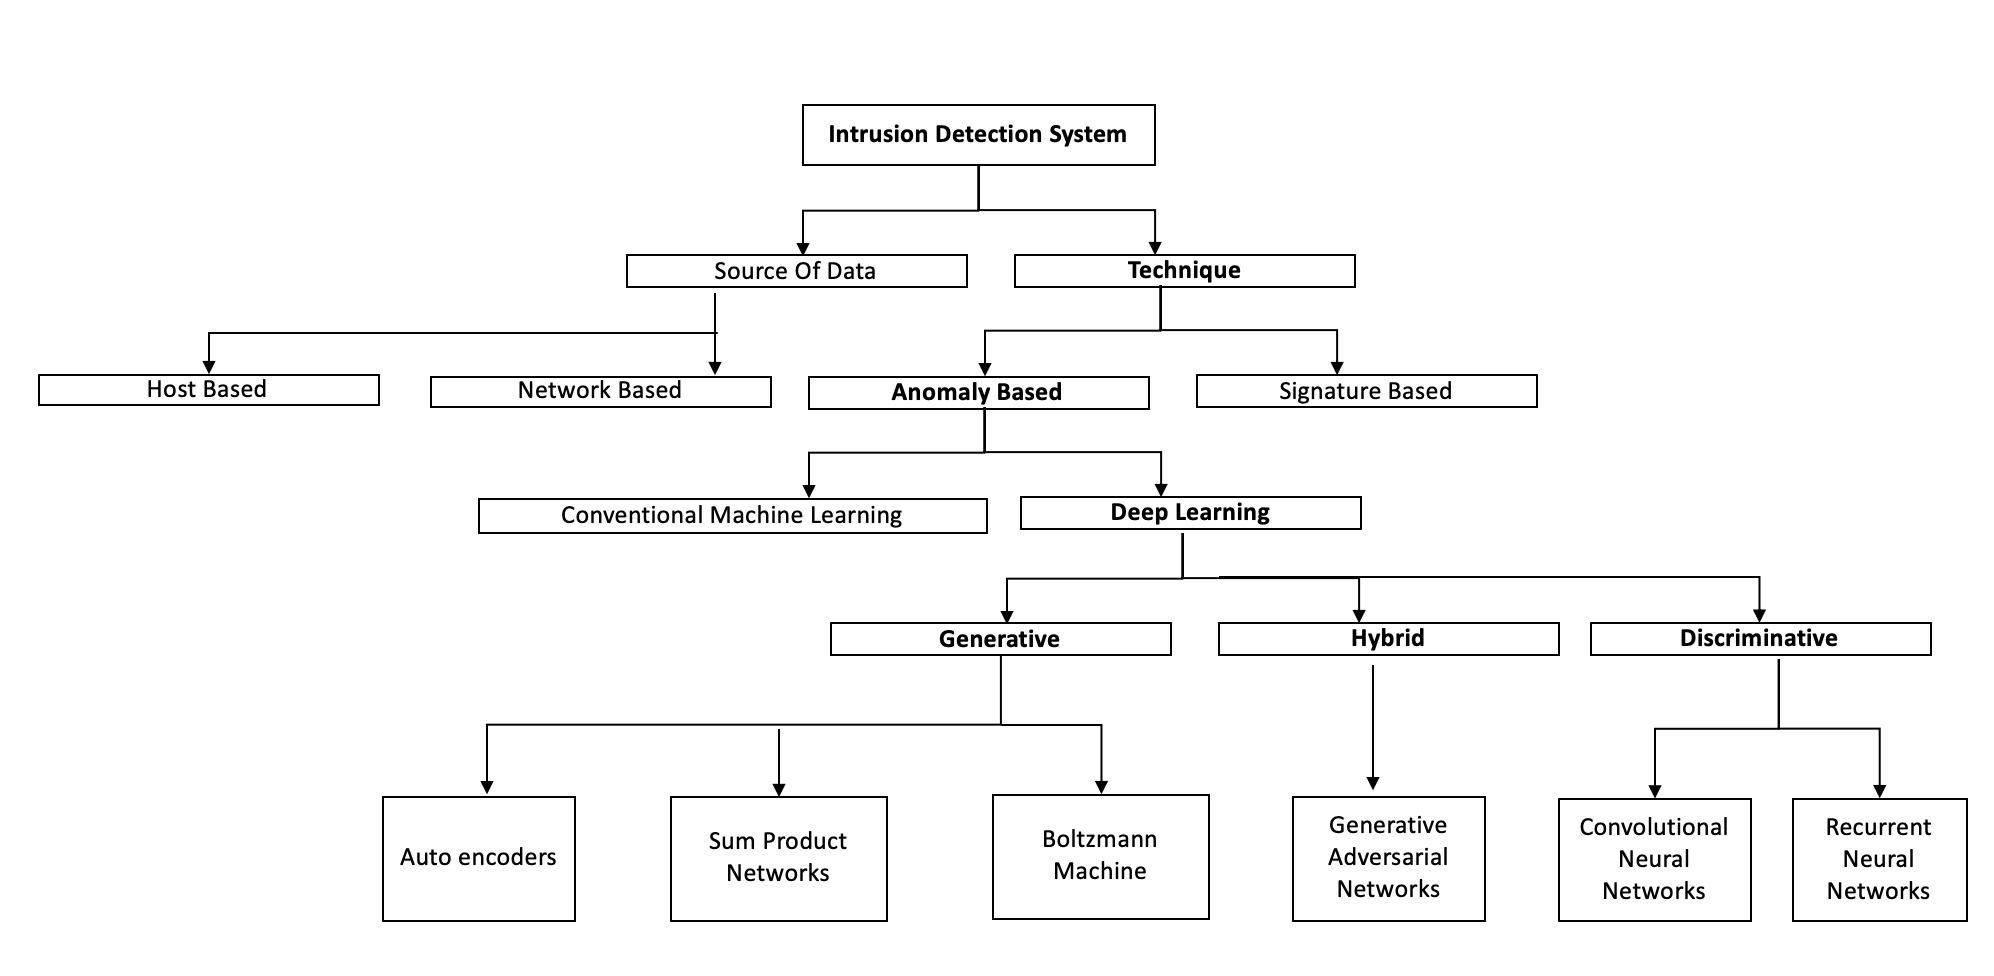
\includegraphics[scale=0.5]{images/IDS}
\captionsetup{justification=centering}
\caption{Classification of deep learning methods for Intrusion Detection.}
\label{fig:deepADforIDS}
\end{figure*}
% End of Figure


%%%%%%% HIDS Network intrusion detection%%%%%%%
%%% Table  Describing the model architectures and techniques used  of HIDS
\begin{table*}
\begin{center}
\caption{Examples of Deep learning anomaly detection Techniques Used in HIDS
          \\CNN: Convolution Neural Networks, LSTM : Long Short Term Memory Networks
          \\GRU: Gated Recurrent Unit, DNN : Deep Neural Networks
          \\SPN: Sum Product Networks}
  \label{tab:HIDS}
    \begin{tabular}{ | l | p{4cm} | l | p{5cm} |}
    \hline
    Techniques & Model Architecture & Section & References \\ \hline
    Discriminative &  LSTM , CNN-LSTM-GRU, DNN & Section ~\ref{sec:rnn_lstm_gru},~\ref{sec:cnn},~\ref{sec:dnn} &  ~\cite{kim2016lstm},~\cite{chawla2018host},~\cite{chen2018henet},~\cite{sohi2018recurrent},~\cite{vinayakumar2017applying} \\\hline
    Hybrid &  GAN & Section ~\ref{sec:hybridModels} & ~\cite{aghakhani2018detecting}, ~\cite{li2018anomaly} \\\hline
    Generative &  AE, SPN,  & Section ~\ref{sec:ae},~\ref{sec:spn} & ~\cite{gao2014intrusion},~\cite{peharz2018probabilistic},~\cite{umer2018two} \\
    \hline
    \end{tabular}
\end{center}
\end{table*}
%%%% End of Table NIDS




%%% Host based Intrusion detection system table%%%%%%
%%% Table  Describing the model architectures and techniques used  of NIDS
\begin{table*}
\begin{center}
  \caption{Examples of Deep learning anomaly detection Techniques Used in NIDS.
          \\CNN: Convolution Neural Networks, LSTM : Long Short Term Memory Networks
          \\RNN: Recurrent Neural Networks, RBM : Restricted Boltzmann Machines
          \\DCA: Dilated Convolution Autoencoders, CVAE : Convolutional Variational Autoencoder
          \\AE: Autoencoders, SAE: Stacked Autoencoders , DBN : Deep Belief Network
          \\GAN: Generative Adversarial Networks. }
  \label{tab:NIDS}
    \begin{tabular}{ | l | p{4cm} | l | p{5cm} |}
    \hline
    Techniques & Model Architecture & Section & References \\ \hline
   Generative  & DCA, SAE, RBM, DBN, CVAE & Section ~\ref{sec:cnn},~\ref{sec:ae},~\ref{sec:dnn},~\ref{sec:gan_adversarial} & ~\cite{yu2017network},~\cite{thing2017ieee}, ~\cite{zolotukhin2016increasing},~\cite{cordero2016analyzing},~\cite{alrawashdeh2016toward},~\cite{tang2016deep},~\cite{lopez2017conditional},~\cite{al2018deep},~\cite{mirsky2018kitsune},~\cite{aygun2017network} \\ \hline
  Hybrid  & GAN   & Section ~\ref{sec:hybridModels} & ~\cite{lin2018idsgan},~\cite{yin2018enhancing}, ~\cite{ring2018flow}, ~\cite{latah2018deep},~\cite{intrator2018mdgan},~\cite{matsubara2018anomaly},~\cite{nicolau2016hybrid} ,~\cite{rigaki2017adversarial}. \\ \hline
  Discriminative &  RNN , LSTM ,CNN & Section ~\ref{sec:rnn_lstm_gru},Section ~\ref{sec:cnn} & ~\cite{yu2017network}, ~\cite{malaiya2018empirical} ~\cite{kwon2018empirical},~\cite{gao2014intrusion},~\cite{staudemeyer2015applying},~\cite{naseer2018enhanced}\\
  \hline
  \end{tabular}
\end{center}
\end{table*}
%%%% End of Table NIDS


% Datasets Used Table
%%% Host based Intrusion detection system table%%%%%%
%%% Table  Describing the model architectures and techniques used  of NIDS
\begin{table*}
\begin{center}
  \caption{Datasets Used in Intrusion Detection }
   \label{tab:IDSDataset}
    \begin{tabular}{ | p{3cm} | l | p{5cm} | l | p{5cm} |}
    \hline
    DataSet &IDS & Description & Type & References \\ \hline
    CTU-UNB & NIDS & CTU-UNB~\cite{ucsdAnomalyDetect2017} dataset consists of various botnet traffics from CTU-13 dataset [20] and normal traffics from the UNB ISCX IDS 2012 dataset ~\cite{shiravi2012toward}  & Hexadecimal & ~\cite{yu2017network} \\ \hline
    Contagio-CTU-UNB & NIDS  & Contagio-CTU-UNB dataset consists of six types of network traffic data. ~\cite{adam2008robust}  & Text & ~\cite{yu2017network}. \\ \hline
    NSL-KDD~\footnote{http://nsl.cs.unb.ca/NSL-KDD/}& NIDS &The NSL-KDD data set is a refined version of its predecessor KDD‟99 data set.  ~\cite{ucsdAnomalyDetect2017} & Text &  ~\cite{yin2017deep},~\cite{javaid2016deep},  ~\cite{tang2016deep},~\cite{yousefi2017autoencoder},~\cite{mohammadi2017new}, ~\cite{lopez2017conditional}\\\hline
    DARPA KDD- CUP 99 & NIDS & DARPA KDD~\cite{stolfo2000cost} The competition task was to build a network intrusion detector, a predictive model capable of distinguishing between ``bad'' connections, called intrusions or attacks, and ``good'' normal connections.  & Text   & ~\cite{alrawashdeh2016toward} ,~\cite{van2017anomaly},~\cite{mohammadi2017new}\\\hline
    MAWI& NIDS  & The  MAWI~\cite{fontugne2010mawilab}  dataset  consists  of  network  traffic  capturedfrom  backbone  links  between  Japan  and  USA.  Every  daysince  2007  & Text   & ~\cite{cordero2016analyzing} \\\hline
    Realistic Global Cyber Environment (RGCE) & NIDS & RGCE~\cite{jamkRGCE}  contains
    realistic Internet Service Providers (ISPs) and numerous different web services as
    in the real Internet.  &  Text   & ~\cite{zolotukhin2016increasing} \\\hline
    ADFA-LD& HIDS & The ADFA Linux Dataset (ADFA-LD). This dataset provides a contemporary Linux dataset for evaluation by traditional HIDS~\cite{creech2014semantic} & Text   & ~\cite{kim2016lstm},~\cite{chawla2018host} \\\hline
    UNM-LPR& HIDS & Consists of system calls to evalute HIDS system~\cite{ImmuneDatasets} & Text   & ~\cite{kim2016lstm} \\\hline
    Infected PDF samples& HIDS & Consists of set of Infected PDF samples, which are used to monitor the malicious traffic  & Text   &~\cite{chen2018henet}\\\hline
    \end{tabular}
\end{center}
\end{table*}
%%%% End of Table NIDS












